\documentclass[14pt]{extbook}
\usepackage{multicol, enumerate, enumitem, hyperref, color, soul, setspace, parskip, fancyhdr} %General Packages
\usepackage{amssymb, amsthm, amsmath, bbm, latexsym, units, mathtools} %Math Packages
\everymath{\displaystyle} %All math in Display Style
% Packages with additional options
\usepackage[headsep=0.5cm,headheight=12pt, left=1 in,right= 1 in,top= 1 in,bottom= 1 in]{geometry}
\usepackage[usenames,dvipsnames]{xcolor}
\usepackage{dashrule}  % Package to use the command below to create lines between items
\newcommand{\litem}[1]{\item#1\hspace*{-1cm}\rule{\textwidth}{0.4pt}}
\pagestyle{fancy}
\lhead{Makeup Progress Quiz 3}
\chead{}
\rhead{Version C}
\lfoot{4315-3397}
\cfoot{}
\rfoot{Fall 2020}
\begin{document}

\begin{enumerate}
\litem{
Solve the rational equation below. Then, choose the interval(s) that the solution(s) belongs to.\[ \frac{3}{-7x + 9} + -2 = \frac{9}{-42x + 54} \]\begin{enumerate}[label=\Alph*.]
\item \( \text{All solutions lead to invalid or complex values in the equation.} \)
\item \( x \in [0.18,2.18] \)
\item \( x_1 \in [0.2, 1.6] \text{ and } x_2 \in [1.45,2.01] \)
\item \( x \in [-2.1,-0.2] \)
\item \( x_1 \in [-2.1, -0.2] \text{ and } x_2 \in [1.09,1.32] \)

\end{enumerate} }
\litem{
Solve the rational equation below. Then, choose the interval(s) that the solution(s) belongs to.\[ \frac{-2x}{-5x + 5} + \frac{-3x^{2}}{20x^{2} -20} = \frac{5}{-4x -4} \]\begin{enumerate}[label=\Alph*.]
\item \( x_1 \in [-0.31, 5.69] \text{ and } x_2 \in [-3,4] \)
\item \( \text{All solutions lead to invalid or complex values in the equation.} \)
\item \( x \in [-6,0] \)
\item \( x \in [-7.29,-3.29] \)
\item \( x_1 \in [-0.31, 5.69] \text{ and } x_2 \in [-10.29,-4.29] \)

\end{enumerate} }
\litem{
Choose the graph of the equation below.\[ f(x) = \frac{1}{(x - 3)^2} - 2 \]\begin{enumerate}[label=\Alph*.]
\begin{multicols}{2}\item 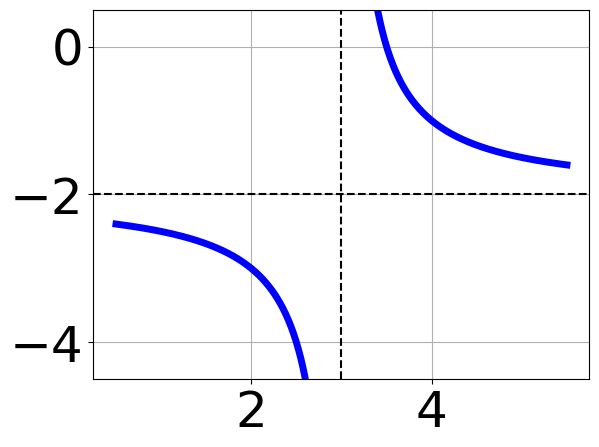
\includegraphics[width = 0.3\textwidth]{../Figures/rationalEquationToGraphCopyAC.png}\item 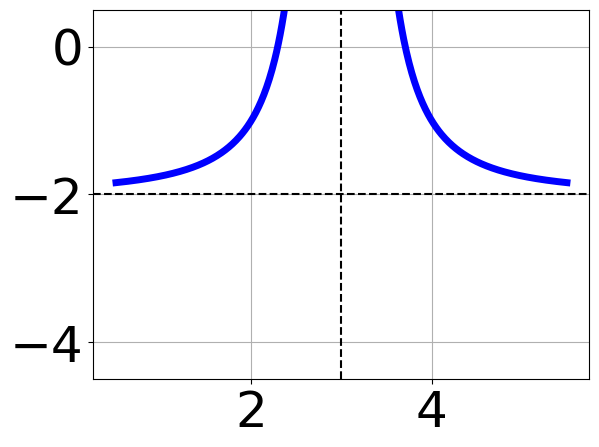
\includegraphics[width = 0.3\textwidth]{../Figures/rationalEquationToGraphCopyBC.png}\item 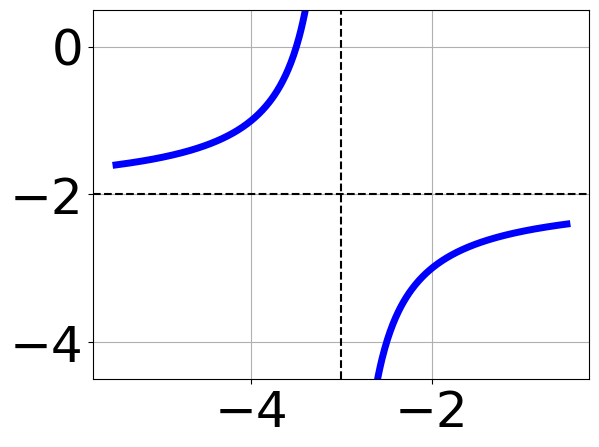
\includegraphics[width = 0.3\textwidth]{../Figures/rationalEquationToGraphCopyCC.png}\item 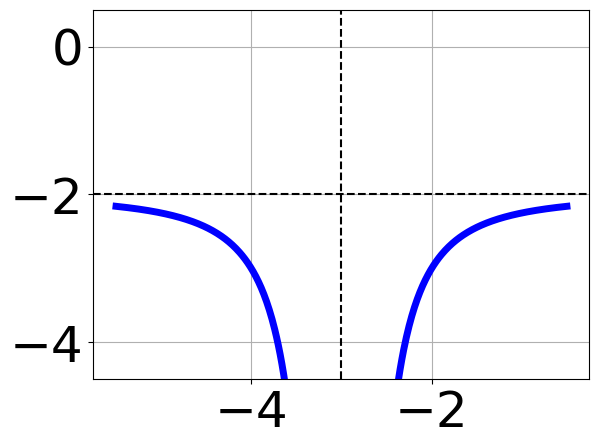
\includegraphics[width = 0.3\textwidth]{../Figures/rationalEquationToGraphCopyDC.png}\end{multicols}\item None of the above.
\end{enumerate} }
\litem{
Determine the domain of the function below.\[ f(x) = \frac{3}{15x^{2} +43 x + 30} \]\begin{enumerate}[label=\Alph*.]
\item \( \text{All Real numbers except } x = a, \text{ where } a \in [-30.13, -29.84] \)
\item \( \text{All Real numbers.} \)
\item \( \text{All Real numbers except } x = a \text{ and } x = b, \text{ where } a \in [-1.67, -1.48] \text{ and } b \in [-1.3, -1.2] \)
\item \( \text{All Real numbers except } x = a, \text{ where } a \in [-1.67, -1.48] \)
\item \( \text{All Real numbers except } x = a \text{ and } x = b, \text{ where } a \in [-30.13, -29.84] \text{ and } b \in [-15.09, -14.76] \)

\end{enumerate} }
\litem{
Choose the equation of the function graphed below.
\begin{center}
    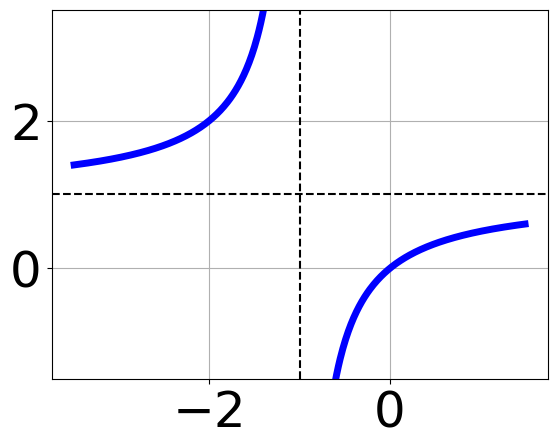
\includegraphics[width=0.5\textwidth]{../Figures/rationalGraphToEquationC.png}
\end{center}
\begin{enumerate}[label=\Alph*.]
\item \( f(x) = \frac{-1}{(x + 1)^2} + 1 \)
\item \( f(x) = \frac{-1}{x + 1} + 1 \)
\item \( f(x) = \frac{1}{(x - 1)^2} + 1 \)
\item \( f(x) = \frac{1}{x - 1} + 1 \)
\item \( \text{None of the above} \)

\end{enumerate} }
\litem{
Determine the domain of the function below.\[ f(x) = \frac{6}{12x^{2} -25 x + 12} \]\begin{enumerate}[label=\Alph*.]
\item \( \text{All Real numbers.} \)
\item \( \text{All Real numbers except } x = a \text{ and } x = b, \text{ where } a \in [11.2, 12.4] \text{ and } b \in [11.2, 12.4] \)
\item \( \text{All Real numbers except } x = a \text{ and } x = b, \text{ where } a \in [0.2, 1.2] \text{ and } b \in [0.9, 2.1] \)
\item \( \text{All Real numbers except } x = a, \text{ where } a \in [11.2, 12.4] \)
\item \( \text{All Real numbers except } x = a, \text{ where } a \in [0.2, 1.2] \)

\end{enumerate} }
\litem{
Solve the rational equation below. Then, choose the interval(s) that the solution(s) belongs to.\[ \frac{3x}{-3x + 3} + \frac{-7x^{2}}{-9x^{2} +30 x -21} = \frac{-4}{3x -7} \]\begin{enumerate}[label=\Alph*.]
\item \( x \in [1.68,2.41] \)
\item \( x \in [15.89,16.77] \)
\item \( x_1 \in [-2.06, 1.97] \text{ and } x_2 \in [10.13,24.13] \)
\item \( x_1 \in [-2.06, 1.97] \text{ and } x_2 \in [-3,7] \)
\item \( \text{All solutions lead to invalid or complex values in the equation.} \)

\end{enumerate} }
\litem{
Solve the rational equation below. Then, choose the interval(s) that the solution(s) belongs to.\[ \frac{-9}{-8x -7} + 8 = \frac{-9}{-64x -56} \]\begin{enumerate}[label=\Alph*.]
\item \( x \in [-2.0,1.0] \)
\item \( x_1 \in [-1, 0] \text{ and } x_2 \in [-2.1,0.3] \)
\item \( \text{All solutions lead to invalid or complex values in the equation.} \)
\item \( x \in [0.75,3.75] \)
\item \( x_1 \in [-1, 0] \text{ and } x_2 \in [0.2,0.9] \)

\end{enumerate} }
\litem{
Choose the equation of the function graphed below.
\begin{center}
    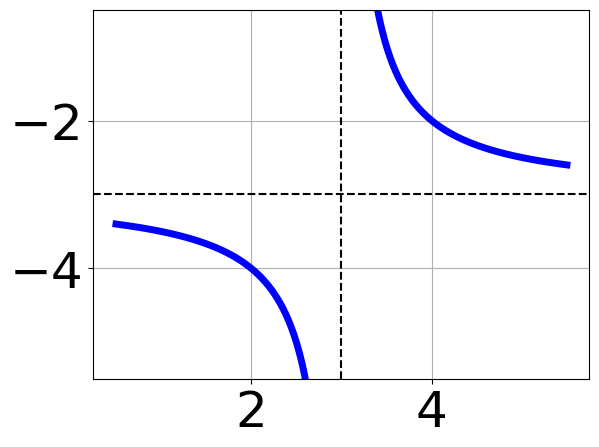
\includegraphics[width=0.5\textwidth]{../Figures/rationalGraphToEquationCopyC.png}
\end{center}
\begin{enumerate}[label=\Alph*.]
\item \( f(x) = \frac{-1}{x - 3} - 3 \)
\item \( f(x) = \frac{1}{(x + 3)^2} - 3 \)
\item \( f(x) = \frac{-1}{(x - 3)^2} - 3 \)
\item \( f(x) = \frac{1}{x + 3} - 3 \)
\item \( \text{None of the above} \)

\end{enumerate} }
\litem{
Choose the graph of the equation below.\[ f(x) = \frac{1}{x + 2} + 3 \]\begin{enumerate}[label=\Alph*.]
\begin{multicols}{2}\item 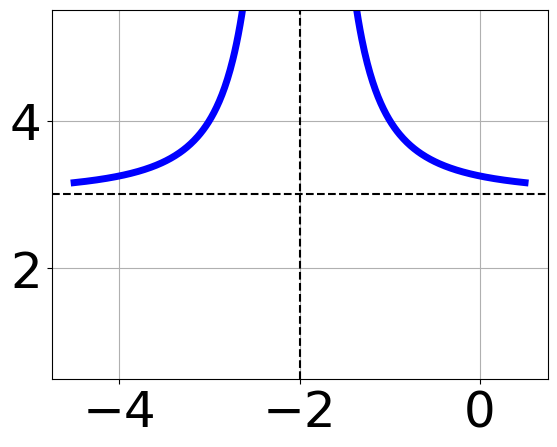
\includegraphics[width = 0.3\textwidth]{../Figures/rationalEquationToGraphAC.png}\item 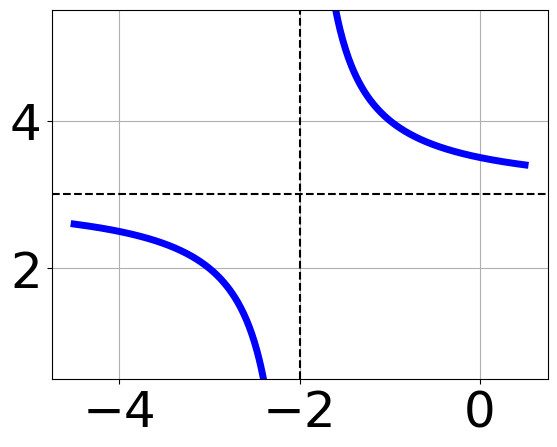
\includegraphics[width = 0.3\textwidth]{../Figures/rationalEquationToGraphBC.png}\item 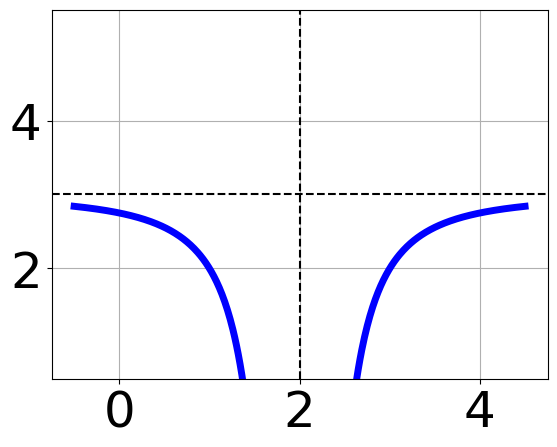
\includegraphics[width = 0.3\textwidth]{../Figures/rationalEquationToGraphCC.png}\item 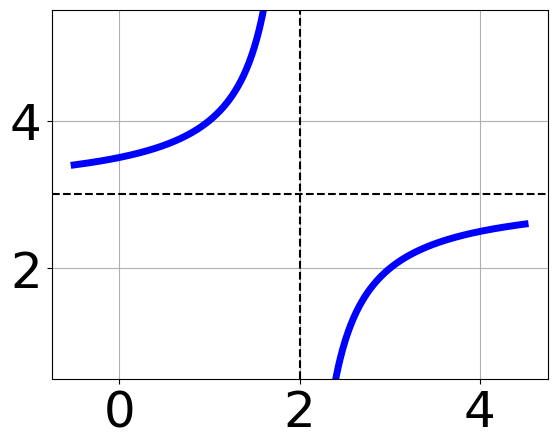
\includegraphics[width = 0.3\textwidth]{../Figures/rationalEquationToGraphDC.png}\end{multicols}\item None of the above.
\end{enumerate} }
\end{enumerate}

\end{document}